\section{Module nhận diện địa điểm trực quan - VPR}
Module VPR của pipeline được phát triển dựa trên mô hình MixVPR được giới thiệu trong bài \cite{alibey2023mixvpr}. Đây là một phương pháp tổng hợp đặc trưng. Từ kết quả đặc trưng xác định được từ mô hình backbone, MixVPR giới thiệu một phương pháp tổng hợp mới, được thực hiện bởi khối Feature Mixer, một cấu trúc đặc biệt được xây dựng dựa trên mô hình MLP-Mixer \cite{tolstikhin2021mlpmixer}. Mô hình MixVPR sử dụng những khối này nhằm tích hợp thông tin toàn cục vào các đặc trưng. Nhờ vào kiến trúc nhẹ của khối Feature Mixer, hướng tiếp cận này cho phép MixVPR đạt hiệu năng cao ở tập dữ liệu thành thị phạm vi rộng mà không có tác động tài nguyên lớn.

\subsection{Kiến trúc}

\begin{figure}[H]
    \centering
    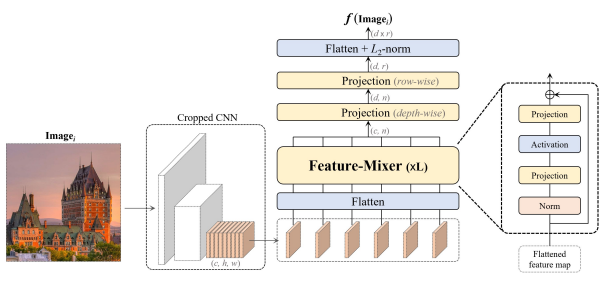
\includegraphics[width=\textwidth]{pics/Proposal/mixvpr.png}
    \caption{Tổng quan quá trình hoạt động của MixVPR \cite{alibey2023mixvpr}}
\end{figure}

\subsubsection{Mô hình backbone trích xuất đặc trưng thô}
Khi ảnh truy vấn $I$ được đưa vào, mô hình CNN backbone được sử dụng để trích xuất ra những chi tiết mang thông tin cần thiết. Mô hình cơ sở được huấn luyện trên những tập dữ liệu hình ảnh đa dạng, nhằm có thể phát hiện ra những đặc trưng quan trọng phục vụ các tác vụ liên quan đến thị giác máy tính. Trong kiến trúc đề xuất, mô hình cơ sở được cắt ở giữa, nhằm thu được tập những bản đồ đặc trưng $F$ có định dạng $F \in R^{c \cdot h \cdot w}$.

Ở những phương pháp trước đây như NetVLAD \cite{arandjelovic2016netvlad} và PatchNetVLAD \cite{hausler2021patchnetvlad}, những lớp bản đồ đặc trưng thuộc $F$ được xem như là một mô tả tương ứng với một miền tiếp nhận cho một khu vực trong ảnh ban đầu. Ngược lại, MixVPR xem $F$ như một tập các bản đồ đặc trưng 2D có kích thước $h \cdot w$, miêu tả toàn ảnh. Đây là một cách biểu diễn ảnh nhỏ, nhẹ và thống nhất hơn trong điều kiện thay đổi về ánh sáng và góc nhìn, thay cho việc lưu trữ từng điểm ảnh.
\begin{equation}
    F = \{X^{i}\},
\end{equation}
với $i \in \left[1,..,c\right]$ và $X^{i}$ tương ứng với bản đồ kích hoạt thứ $i$ ở F.

Mỗi bản đồ đặc trưng $X^{i}$ thuộc tập $F$ sau đó được được định dạng lại thành ma trận một chiều có dạng $X_{flat}^{i} \in R^{h*w}$, thu được được $F_{flat} \in R^{c \cdot n}$ với $n = h*w$.

\subsubsection{Khối tổng hợp Feature Mixer}
Tiếp theo, tập hợp của những bản đồ đặc trưng $F_{flat}$ lần lượt được đưa qua $L$ khối Feature Mixer, được phát triển trên cấu trúc mạng MLP. Mỗi khối Feature Mixer nhận vào từng bản đồ đặc trưng $X_{flat}^{i}$ một chiều và tích hợp thông tin về mối liên kết giữa các giá trị của $X_{flat}^{i}$ lên chính nó thông qua cách sau:
\begin{equation}
    \begin{aligned}
        X^{i} & \leftarrow Norm(X^{i})             \\
        X^{i} & \leftarrow W_2(\sigma(W_1 X^{i})),
    \end{aligned}
\end{equation}
với $W_1$ và $W_2$ là trọng số của hai lớp liên kết đầy đủ, cấu tạo nên MLP và $\sigma$ là hàm tạo sự phi tuyến tính cho quá trình xử lý (ReLU). Kỹ thuật nối tắt được sử dụng để nối đầu vào đã qua lớp chuẩn hóa với đầu ra nhằm giúp độ dốc trong quá trình huấn luyện có thể được truyền tải dễ hơn, cải thiện quá trình huấn luyện. Kết quả đầu ra của khối Feature Mixer được giữ định dạng giống như dữ liệu đầu vào, có dạng $R^{h*w}$.

Mục đích của việc sử dụng Feature Mixer là để tận dụng khả năng tổng hợp thông tin từ dữ liệu của các lớp kết nối đầy đủ, thay vì học trên những đặc trưng cục bộ trên ảnh và sử dụng cơ chế tập trung. Ngoài ra, Feature Mixer cũng trả về kết quả có định dạng và kích thước như đầu vào, thay vì giảm dần như những phương pháp tổng hợp dạng phân cấp (kim tự tháp) như trước đây, để mỗi neuron đều có thể biết được thông tin của toàn bộ ảnh. Những lớp MLP trong khối Feature Mixer giúp tích hợp thông tin trên toàn bộ ảnh qua mỗi lần xử lý.

Mỗi khối Feature Mixer sau khi xử lý xong từng bản đồ đặc trưng trong tập $F_{flat} \in R^{c \cdot n}$ ghép kết quả lại, tạo thành $Z \in R^{c \cdot n}$ với cùng kích thước trước khi được đưa vào khối Feature Mixer kế tiếp. Quá trình xử lý tập bản đồ đặc trưng qua các khối Feature Mixer có thể được miêu tả bằng công thức sau:
\begin{equation}
    Z = FM_L(FM_{L-1}(\dots FM_1(F_{flat}))),
\end{equation}
với $FM_i$ là lớp Feature Mixer thứ $i$ trên tổng số $L$ khối và $Z$ là kết quả cuối cùng của quá trình tích hợp thông tin toàn cục.

\subsubsection{Lớp tổng hợp - Aggregation}
Ta có $Z \in R^{c \cdot n}$ với số chiều rất cao do có định dạng được giữ nguyên so với $F_{flat}$. Để giúp giảm bớt số chiều của $Z$ lại sau khi qua khối Feature Mixer, hai lớp kết nối đầy đủ được sử dụng để thực hiện tác vụ tổng hợp lần lượt giữa các giá trị trên cùng một kênh $c$ với nhau và sau đó là giữa các giá trị trong từng bản đồ đặc trưng $X_{flat}^i$. Tác vụ này thực hiện việc tổng hợp có chọn lọc nhằm điều khiển được kích thước của giá trị đầu ra.

Đầu tiên, dữ liệu được tổng hợp số kênh để biến định dạng của $Z$ từ $R^{c \cdot n}$ thành $R^{d \cdot n}$.
\begin{equation}
    Z' = W_d(Transpose(Z)),
\end{equation}
với $W_d$ là trọng số của lớp kết nối đầy đủ đầu tiên và $d$ là định dạng đầu ra sau khi rút gọn số kênh lại, $d<c$.

Sau đó, giá trị trên từng bản đồ đặc trưng được tổng hợp lại, từ định dạng $R^{d \cdot n}$ thành $R^{d \cdot r}$.
\begin{equation}
    O = W_r(Transpose(Z')),
\end{equation}
với $W_r$ là trọng số của lớp kết nối đầy đủ thứ hai và $r$ là định dạng đầu ra của các bản đồ đặc trưng 1D, $r<n$.

Kết quả $O$ cuối cùng, có định dạng là $R^{d \cdot r}$, được ép thành một chiều và chuẩn hóa theo $L_2$ như những phương pháp VPR khác \cite{arandjelovic2016netvlad,berton2022rethinking}. Cuối cùng, từ ảnh đầu vào $I$, mô hình trả về một đoạn mã hóa biểu diễn cho nội dung của ảnh. Đoạn mã hóa này sau đó có thể được dùng để so sánh với giá trị mã hóa của những hình khác nhằm tìm ảnh có độ tương đồng cao nhất với $I$.

\subsubsection{Bộ phận truy xuất ảnh tương đồng}
Sau khi đã có được giá trị mã hóa biễu diễn cho ảnh truy vấn là $O \in R^{d \cdot r}$, mô hình tiến hành tìm kiếm trên tập dữ liệu ảnh miêu tả khu vực đang xét. Cơ chế tìm kiếm được sử dụng là tìm kiếm toàn diện, xét giá trị biểu diễn của từng ảnh. $k$ ảnh có độ tương đồng cao nhất với ảnh truy vấn được chọn để tạo thành các cặp ảnh là đầu ra của bước này.

\begin{figure}[H]
    \centering
    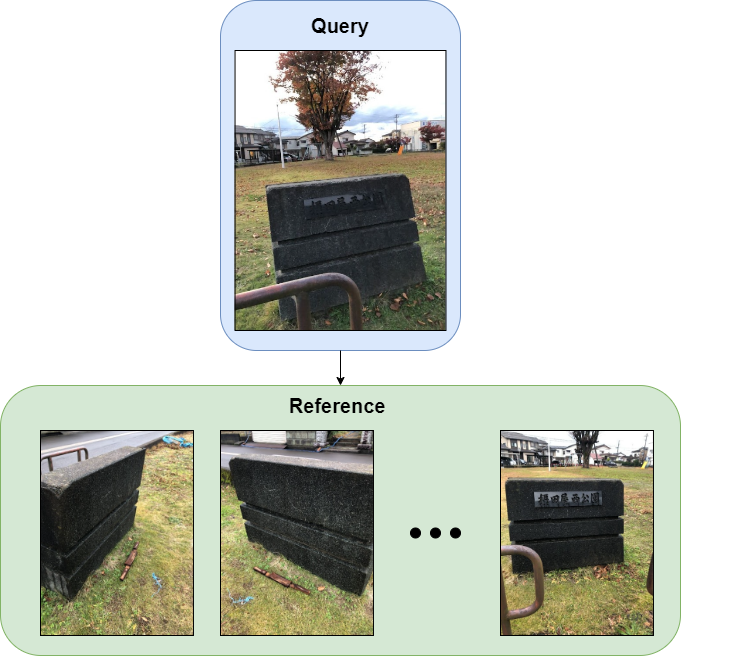
\includegraphics[scale=0.4]{pics/Proposal/query.png}
    \caption[Kết quả của module VPR]{Ảnh truy xuất được từ ảnh truy vấn $I$ ban đầu, từ tập dữ liệu Niantic \cite{arnold2022mapfree}}
\end{figure}


\subsection{Phương pháp hiện thực và triển khai}

\subsubsection{Hiện thực}

Mô hình MixVPR được hiện thực trên framework PyTorch. Mô hình CNN cơ sở của MixVPR được cắt ở lớp áp cuối của mô hình ResNet. Dữ liệu đầu vào cho MixVPR là các ảnh đã được chỉnh về độ phân giải $320x320$ và qua mô hình backbone, một tập các bản đồ đặc trưng có kích thước 20x20 được đưa vào tập $L$ khối Feature Mixer. Thao tác tổng hợp trong khối Feature Mixer sử dụng lớp Linear, theo sau đó là một lớp ReLU để tạo tính phi tuyến tính. Về lớp chuẩn hóa, LayerNorm được sử dụng. Cuối cùng, đầu ra cuối cùng của khối Feature Mixer được tổng hợp xuống một chiều không gian biểu diễn nhỏ hơn sử dụng hai lớp kết nối đầy đủ giữa các kênh với nhau và giữa các giá trị trong mỗi kênh, chứng minh rằng MixVPR là một cấu trúc chỉ sử dụng MLP. Số khối Feature Mixer được sử dụng mặc định là $L=4$.

\subsubsection{Huấn luyện}
Mô hình MixVPR được đánh giá trong bài nghiên cứu sử dụng mô hình ResNet \cite{he2016deep} đã được huấn luyện trên tập ImageNet \cite{krizhevsky2012imagenet} làm cơ sở. Sau đó, mô hình được huấn luyện trên tập dữ liệu GSV-Cities \cite{Ali_bey_2022}. Đối với hàm mất mát, hàm Multi-Similarity Loss \cite{wang2019multi} được sử dụng với lý do đã được chứng minh là hỗ trợ cho ra kết quả tốt nhất với tác vụ VPR \cite{Ali_bey_2022}. Kích thước của một batch có $P = 120$ địa điểm, mỗi địa điểm được miêu tả bởi 4 ảnh, tạo thành một batch có kích thước 480 ảnh. Phương pháp tối ưu giảm độ dốc ngẫu nhiên - SGD được sử dụng với quán tính - momentum là 0.9 với giá trị suy giảm trọng số - weight decay là 0.001. Tốc độ học - learning rate được khởi tạo với giá trị 0.05 và được chia 3 sau mỗi 5 chu kỳ - epoch. Cuối cùng, mô hình được huấn luyện tối đa 30 chu kỳ - epoch với đầu vào là ảnh đã được điều chỉnh kích thước 320x320.

\subsubsection{Phương pháp đánh giá}
Để đánh giá hiệu năng mô hình, 5 tập dữ liệu tiêu chuẩn đã được sử dụng. Pitts250k-test \cite{6618963}, bao gồm 8.000 ảnh truy vấn và 83.000 ảnh tham khảo, được thu thập từ Google Street View và Pitts30k-test \cite{6618963} là một tập con của Pitts250k bao gồm 8.000 ảnh truy vấn và 8.000 ảnh tham khảo. Cả 2 tập dữ liệu Pittsburgh đều có những góc nhìn có độ lệch đáng kể, những chi tiết kiến trúc tương đồng cũng thường xuyên xuất hiện trong tập dữ liệu này. Tập dữ liệu SPEDTest \cite{zaffar2021vpr} gồm 607 ảnh truy vấn và 607 ảnh tham khảo thu từ camera giám sát, chứa những thay đổi lớn về độ sáng và về cảnh vật các mùa. MSLS \cite{warburg2020mapillary} được thu thập từ camera hành trình của xe hơi, cho rất nhiều góc nhìn đa dạng cũng như đa dạng về sự thay đổi độ sáng. Cuối cùng, Nordland \cite{zaffar2021vpr} là một tập dữ liệu chứa nhiều thử thách khi sử dụng ảnh thu thập được ở cả 4 mùa với camera được gắn trên tàu. Đơn vị đánh giá được sử dụng là recall@k, thể hiện tỷ lệ của truy xuất thành công trên tổng số lượng truy xuất. Một truy xuất hình được xem là thành công khi ảnh được truy xuất nằm trong vòng 25m xung quanh ảnh truy vấn.

\subsection{Kết quả}
Khi so sánh trên những tập dữ liệu phản ánh môi trường thành thị, mô hình MixVPR đạt được kết quả vượt trội so với những mô hình SOTA đã được đề xuất trước nó, như CosPlace \cite{berton2022rethinking} và NetVLAD \cite{arandjelovic2016netvlad}. Những tập dữ liệu được sử dụng đã bao quát hết những trường hợp có thể tác động xấu đến mô hình như góc nhìn đa dạng; thời tiết, mùa thay đổi; chênh lệch về độ sáng. MixVPR cũng có khả năng giải quyết được những trường hợp mà những phương pháp trước gặp khó khăn như: kiến trúc lặp lại nhiều, góc nhìn thay đổi rõ rệt, đường chân trời, độ sáng chênh lệch lớn và gặp nhiều vật thể cản trở tầm nhìn. Tuy nhiên, mô hình vẫn gặp thất bại khi độ chênh lệch góc nhìn là quá lớn hoặc có quá nhiều vật cản. Những trường hợp thất bại của mô hình MixVPR được thể hiện ở hình \textbf{3.5}

\begin{figure}
    \centering
    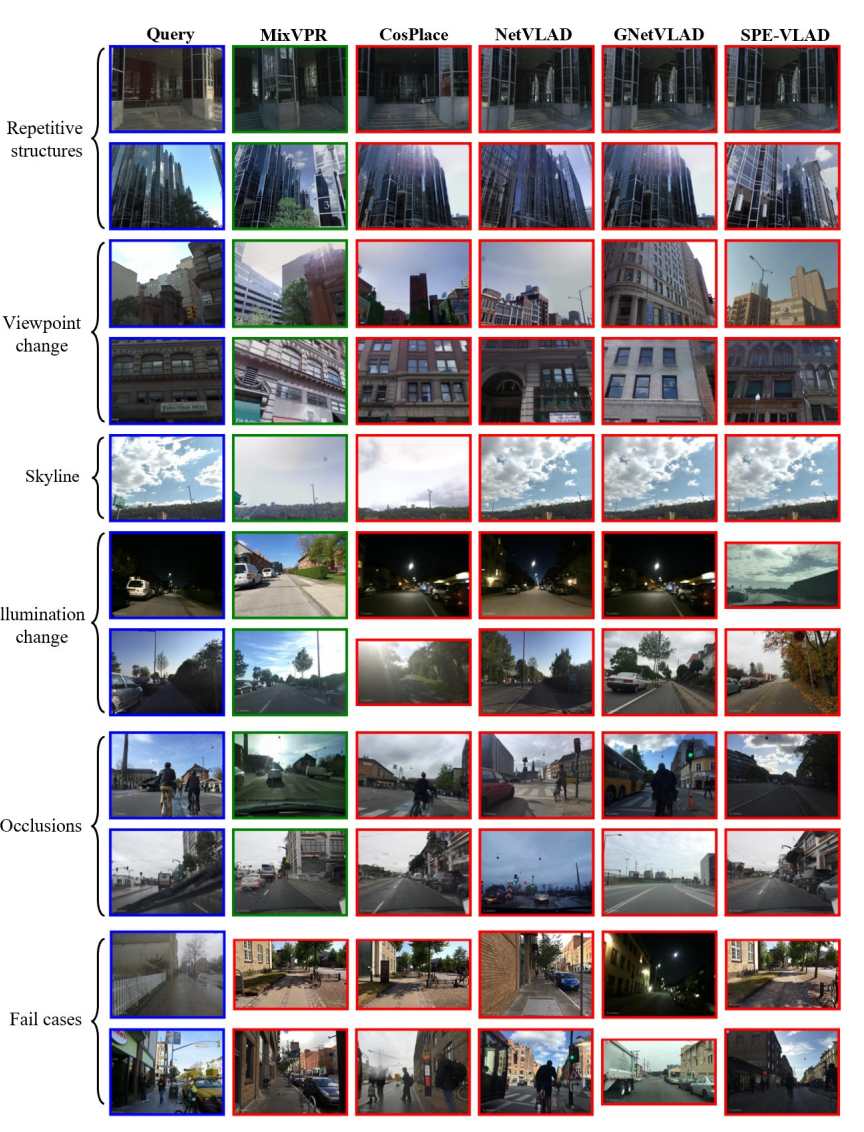
\includegraphics[width=\textwidth]{pics/Proposal/fail.png}
    \caption{Kết quả của những trường hợp khó khi chạy trên MixVPR và các phương pháp khác \cite{alibey2023mixvpr}}
\end{figure}

Với sự ra đời của AnyLoc \cite{keetha2023anyloc}, bài toán VPR trong những môi trường đa dạng hơn như trong nhà, trong hang động, trên bầu trời, hoặc trên mặt biển đã có một SOTA mới. Điều này là nhờ việc AnyLoc sử dụng mạng cơ sở DINO, một mạng Vision Transformer được huấn luyện bằng cơ chế tự giám sát để sinh ra những đặc trưng có giá trị với mọi tác vụ. Tuy nhiên, khi xét đến môi trường thành thị thì MixVPR vẫn có cho ra kết quả chính xác hơn AnyLoc. Số liệu cụ thể được trình bày bên dưới.

% \begin{figure}[H]
%   \centering
%   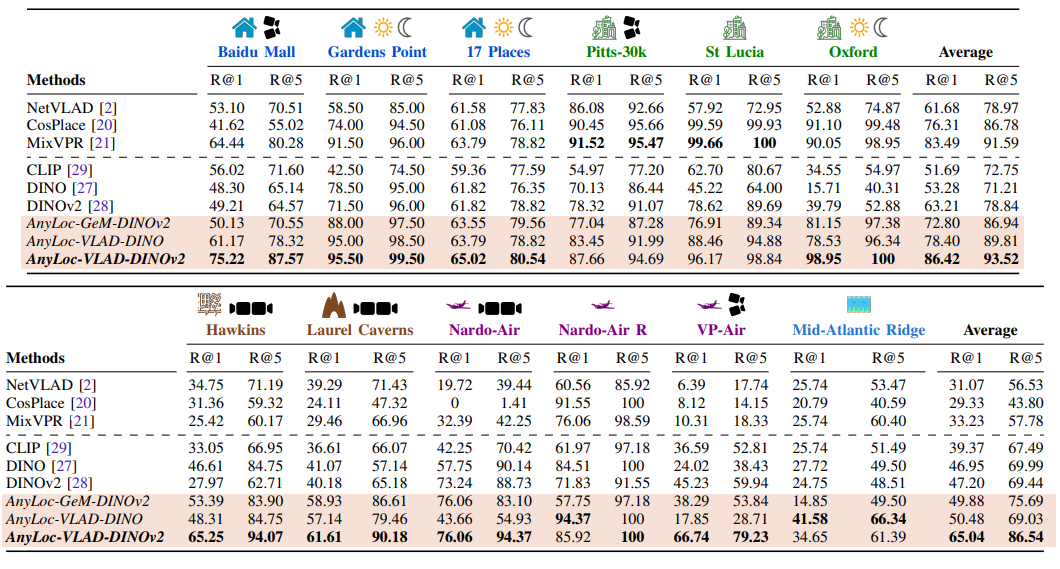
\includegraphics[scale=0.5]{pics/Proposal/anyloc.png}
%   \caption{Kết quả của AnyLoc so sánh với những mô hình khác \cite{keetha2023anyloc}}
% \end{figure}


\begin{table}[H]
    \adjustbox{max width=\textwidth}{
        \begin{tabular}{lcccccccccccccc}
            \cline{2-15}
            \multicolumn{1}{l|}{}                  & \multicolumn{2}{c|}{{\color[HTML]{6434FC} \textbf{Baidu Mall}}} & \multicolumn{2}{c|}{{\color[HTML]{6434FC} \textbf{Gardens Point}}} & \multicolumn{2}{c|}{{\color[HTML]{6434FC} \textbf{17 Places}}} & \multicolumn{2}{c|}{{\color[HTML]{009901} \textbf{Pitts-30k}}} & \multicolumn{2}{c|}{{\color[HTML]{009901} \textbf{St Lucia}}} & \multicolumn{2}{c|}{{\color[HTML]{009901} \textbf{Oxford}}} & \multicolumn{2}{c|}{\textbf{Average}}                                                                                                                                                                                              \\ \hline
            \multicolumn{1}{|l|}{\textbf{Methods}} & \multicolumn{1}{c|}{R@1}                                        & \multicolumn{1}{c|}{R@5}                                           & \multicolumn{1}{c|}{R@1}                                       & \multicolumn{1}{c|}{R@5}                                       & \multicolumn{1}{c|}{R@1}                                      & \multicolumn{1}{c|}{R@5}                                    & \multicolumn{1}{c|}{R@1}              & \multicolumn{1}{c|}{R@5} & \multicolumn{1}{c|}{R@1} & \multicolumn{1}{c|}{R@5} & \multicolumn{1}{c|}{R@1} & \multicolumn{1}{c|}{R@5} & \multicolumn{1}{c|}{R@1} & \multicolumn{1}{c|}{R@5} \\ \hline
            NetVLAD                                & 53.10                                                           & 70.51                                                              & 58.50                                                          & 85.00                                                          & 61.58                                                         & 77.83                                                       & 86.08                                 & 92.66                    & 57.92                    & 72.95                    & 52.88                    & 74.87                    & 61.68                    & 78.97                    \\
            CosPlace                               & 41.62                                                           & 55.02                                                              & 74.00                                                          & 94.50                                                          & 61.08                                                         & 76.11                                                       & 90.45                                 & 95.66                    & 99.59                    & 99.93                    & 91.10                    & 99.48                    & 76.31                    & 86.78                    \\
            MixVPR                                 & 64.44                                                           & 80.28                                                              & 91.50                                                          & 96.00                                                          & 63.79                                                         & 78.82                                                       & \textbf{91.52}                        & \textbf{95.47}           & \textbf{99.66}           & \textbf{100}             & 90.05                    & 98.95                    & 83.49                    & 91.59                    \\ \hline
            CLIP                                   & 56.02                                                           & 71.60                                                              & 42.50                                                          & 74.50                                                          & 59.36                                                         & 77.59                                                       & 54.97                                 & 77.20                    & 62.70                    & 80.67                    & 34.55                    & 54.97                    & 51.69                    & 72.75                    \\
            DINO                                   & 48.30                                                           & 65.14                                                              & 78.50                                                          & 95.00                                                          & 61.82                                                         & 76.35                                                       & 70.13                                 & 86.44                    & 45.22                    & 64.00                    & 15.71                    & 40.31                    & 53.28                    & 71.21                    \\
            DINOv2                                 & 49.21                                                           & 64.57                                                              & 71.50                                                          & 96.00                                                          & 61.82                                                         & 78.82                                                       & 78.32                                 & 91.07                    & 78.62                    & 89.69                    & 39.79                    & 52.88                    & 63.21                    & 78.84                    \\
            \rowcolor[HTML]{FFCE93}
            \textit{AnyLoc-GeM-DINOv2}             & 50.13                                                           & 70.55                                                              & 88.00                                                          & 97.50                                                          & 63.55                                                         & 79.56                                                       & 77.04                                 & 87.28                    & 76.91                    & 89.34                    & 81.15                    & 97.38                    & 72.80                    & 86.94                    \\
            \rowcolor[HTML]{FFCE93}
            \textit{AnyLoc-VLAD-DINO}              & 61.17                                                           & 78.32                                                              & 95.00                                                          & 98.50                                                          & 63.79                                                         & 78.82                                                       & 83.45                                 & 91.99                    & 88.46                    & 94.88                    & 78.53                    & 96.34                    & 78.40                    & 89.81                    \\
            \rowcolor[HTML]{FFCE93}
            \textit{\textbf{AnyLoc-VLAD-DINOv2}}   & \textbf{75.22}                                                  & \textbf{87.57}                                                     & \textbf{95.50}                                                 & \textbf{99.50}                                                 & \textbf{65.02}                                                & \textbf{80.54}                                              & 87.66                                 & 94.69                    & 96.17                    & 98.84                    & \textbf{98.95}           & \textbf{100}             & \textbf{86.42}           & \textbf{93.52}
        \end{tabular}}
    \caption{Bảng so sánh kết quả AnyLoc với những mô hình khác trên những tập dữ liệu thành thị}
\end{table}

\begin{table}[H]
    \adjustbox{max width=\textwidth}{
        \begin{tabular}{lcccccccccccccc}
            \cline{2-15}
            \multicolumn{1}{l|}{}                  & \multicolumn{2}{c|}{{\color[HTML]{986536} \textbf{Hawkins}}} & \multicolumn{2}{c|}{{\color[HTML]{986536} \textbf{Laurel Caverns}}} & \multicolumn{2}{c|}{{\color[HTML]{6200C9} \textbf{Nardo-Air}}} & \multicolumn{2}{c|}{{\color[HTML]{6200C9} \textbf{Nardo-Air R}}} & \multicolumn{2}{c|}{{\color[HTML]{6200C9} \textbf{VP-Air}}} & \multicolumn{2}{c|}{{\color[HTML]{3531FF} \textbf{\begin{tabular}[c]{@{}c@{}}Mid-Atlantic\\ Ridge\end{tabular}}}} & \multicolumn{2}{c|}{\textbf{Average}}                                                                                                                                                                                              \\ \hline
            \multicolumn{1}{|l|}{\textbf{Methods}} & \multicolumn{1}{c|}{R@1}                                     & \multicolumn{1}{c|}{R@5}                                            & \multicolumn{1}{c|}{R@1}                                       & \multicolumn{1}{c|}{R@5}                                         & \multicolumn{1}{c|}{R@1}                                    & \multicolumn{1}{c|}{R@5}                                                                                          & \multicolumn{1}{c|}{R@1}              & \multicolumn{1}{c|}{R@5} & \multicolumn{1}{c|}{R@1} & \multicolumn{1}{c|}{R@5} & \multicolumn{1}{c|}{R@1} & \multicolumn{1}{c|}{R@5} & \multicolumn{1}{c|}{R@1} & \multicolumn{1}{c|}{R@5} \\ \hline
            NetVLAD                                & 34.75                                                        & 71.19                                                               & 39.29                                                          & 71.43                                                            & 19.72                                                       & 39.44                                                                                                             & 60.56                                 & 85.92                    & 6.39                     & 17.74                    & 25.74                    & 53.47                    & 31.07                    & 56.53                    \\
            CosPlace                               & 31.36                                                        & 59.32                                                               & 24.11                                                          & 47.32                                                            & 0                                                           & 1.41                                                                                                              & 91.55                                 & \textbf{100}             & 8.12                     & 14.15                    & 20.79                    & 40.59                    & 29.33                    & 43.80                    \\
            MixVPR                                 & 25.42                                                        & 60.17                                                               & 29.46                                                          & 66.96                                                            & 32.39                                                       & 42.25                                                                                                             & 76.06                                 & 98.59                    & 10.31                    & 18.33                    & 25.74                    & 60.40                    & 33.23                    & 57.78                    \\ \hline
            CLIP                                   & 33.05                                                        & 66.95                                                               & 36.61                                                          & 66.07                                                            & 42.25                                                       & 70.42                                                                                                             & 61.97                                 & 97.18                    & 36.59                    & 52.81                    & 25.74                    & 51.49                    & 39.37                    & 67.49                    \\
            DINO                                   & 46.61                                                        & 84.75                                                               & 41.07                                                          & 57.14                                                            & 57.75                                                       & 90.14                                                                                                             & 84.51                                 & 100                      & 24.02                    & 38.43                    & 27.72                    & 49.50                    & 46.95                    & 69.99                    \\
            DINOv2                                 & 27.97                                                        & 62.71                                                               & 40.18                                                          & 65.18                                                            & 73.24                                                       & 88.73                                                                                                             & 71.83                                 & 91.55                    & 45.23                    & 59.94                    & 24.75                    & 48.51                    & 47.20                    & 69.44                    \\
            \rowcolor[HTML]{FFCE93}
            \textit{AnyLoc-GeM-DINOv2}             & 53.39                                                        & 83.90                                                               & 58.93                                                          & 86.61                                                            & 76.06                                                       & 83.10                                                                                                             & 57.75                                 & 97.18                    & 38.29                    & 53.84                    & 14.85                    & 49.50                    & 49.88                    & 75.69                    \\
            \rowcolor[HTML]{FFCE93}
            \textit{AnyLoc-VLAD-DINO}              & 48.31                                                        & 84.75                                                               & 57.14                                                          & 79.46                                                            & 43.66                                                       & 54.93                                                                                                             & \textbf{94.37}                        & \textbf{100}             & 17.85                    & 28.71                    & \textbf{41.58}           & \textbf{66.34}           & 50.48                    & 69.03                    \\
            \rowcolor[HTML]{FFCE93}
            \textit{\textbf{AnyLoc-VLAD-DINOv2}}   & \textbf{65.25}                                               & \textbf{94.07}                                                      & \textbf{61.61}                                                 & \textbf{90.18}                                                   & \textbf{76.06}                                              & \textbf{94.37}                                                                                                    & 85.92                                 & \textbf{100}             & \textbf{66.74}           & \textbf{79.23}           & 34.65                    & 61.39                    & \textbf{65.04}           & \textbf{86.54}
        \end{tabular}}
    \caption{Bảng so sánh kết quả AnyLoc với những mô hình khác trên những tập dữ liệu ngoài thiên nhiên}
\end{table}